\documentclass[12pt]{article}

% Packages
\usepackage[margin=1in]{geometry}
\usepackage{amsmath, amssymb}
\usepackage{graphicx}
\usepackage{hyperref}
\usepackage{xcolor}
\usepackage{enumitem}
\usepackage{booktabs}
\usepackage{tcolorbox} % For boxes
\tcbset{colback=gray!10, colframe=black, boxrule=0.5pt, arc=4pt}
\usepackage{graphicx} % For inserting images
\usepackage{caption}  % For customizing captions
\usepackage{xcolor} % for colored text





% Custom Commands
\newcommand{\definition}[2]{
    \begin{tcolorbox}
    \textbf{#1:} #2
    \end{tcolorbox}
}
\newcommand{\formula}[2]{
    \begin{tcolorbox}[colback=blue!5!white]
    \textbf{#1:} \[ #2 \]
    \end{tcolorbox}
}


% Custom "lead words" command
\newcommand{\leadwords}[2]{\textcolor{red}{\textbf{\large #1}} #2}

% Paragraph formatting
\setlength{\parindent}{0pt} % No paragraph indentation
\setlength{\parskip}{0.8em} % Space between paragraphs


\title{Introductory Macroeconomics Notes}
\author{Abdullah Yassine}
\date{\today}

\begin{document}

\maketitle
\tableofcontents
\newpage

\section{The Science of Macroeconomics}
\definition{Macroeconomics}{The study of the economy as a whole, focusing on aggregate measures and national policies.}

\subsection{Theory as Model Building}
Children try to learn how the world around them work by playing with little toys. Similarly, economists try to learn how economies work by playing with \textbf{models}. Models often help economists to try to understand the relationship between variables.



Models have two kinds of variables:
\begin{itemize}
    \item \textbf{Endogenous Variables}: variables that a model tries to explain.
    \item \textbf{Exogenous Variables}: variables a model take as given.
\end{itemize}


In other words, models try to explain how exogenous variables affect endogenous variables. Exogenous variables come from outside the model and act as the model's input, whereas endogenous variables are determined within the model and act as the model's output.



\subsection{Prices: Flexbile Versus Sticky}

When creating models, we make assumptions, and we have to keep those assumptions in mind when we make conclusions based on the model. One of the assumptions we make when creating models is \textbf{market clearing} where we assume that whenever something happens to the supply or demand curve, the equilibrium price changes instantly.


In reality, prices and wages stay the same for a long time before changing. For example, job contracts require to pay the same wage rate for 3 years. Magazine companies sell their magazines at the same price for a couple of months before changing those prices.



Market clearing is the best for long-term modelling, while \textbf{market sticky} is best used in short-term modelling.


\section{The Data of Macroeconomics}
% \definition{Gross Domestic Product (GDP)}{The total market value of all final goods and services produced within a country in a given period.}

% \formula{Nominal GDP}{P_t \times Q_t}
% \formula{Real GDP}{P_{\text{base}} \times Q_t}
Now, we learn the tools that are used by macreconomists so they can have a better understanding of the economy.

\definition{Gross Domestic Product (GDP)}{The total market value of all final goods and services produced within a country in a given period. Another definition includes the total income of everyone in the country.}


How is total income the same thing as output produced by the country? When Jill builds a house and sells it to Joe for \$10,000, it's income for Jill but an expenditure to Joe. Regardless, \$10,000 is now part of the GDP.

To better understand this, let's assume a scenario where the economy only produces one product, bread. In this economy, households sell their labor to the firms. Firms use this labor to produce bread which they sell to households. Firms pay money to households for their labor, and households use that money to buy bread from firms. Look at the following figure.


\begin{figure}[h!]
    \centering
    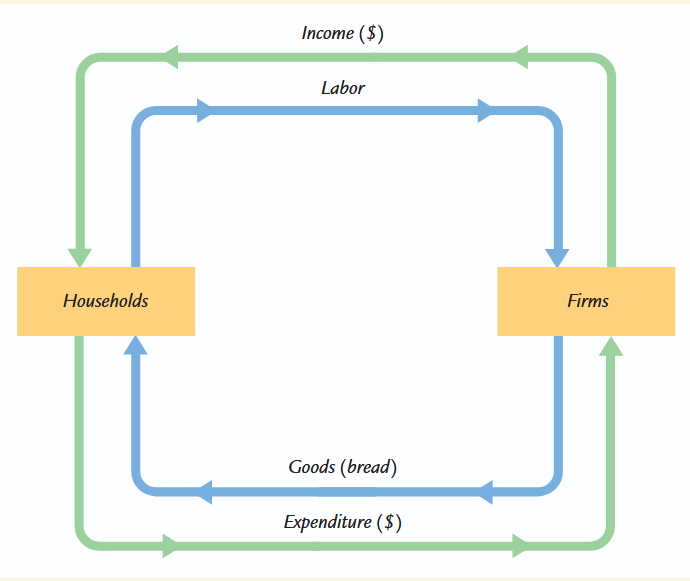
\includegraphics[width=0.75\textwidth]{images/flow.png}
    \caption{The Circular Flow.}
    \label{fig:aggregate_demand}
\end{figure}


So, GDP in this case can be measured in two cases: total income from the production of bread (the top loop), or the total expenditure on purchases of bread (the bottom loop).


\subsection{Measuring the Value of Economic Activity: Gross Domestic Product}


When an economy gets complicated and starts to sell many stuff, how do we calculate GDP now? Just like before, but this time, we use the \textit{market price} because these prices reflect how much people are willing to pay for a good or service.



\leadwords{Used Goods} When it comes to used goods, like someone reselling a pack of basketball cards, that does not go to the GDP because GDP is all about \textit{currently} produced goods and services. This is just a transfer of assets.


\leadwords{The Treatment of Inventories} Let's assume that the firm now produced more bread, which required hiring more workers and increasing wage rates. But nobody buys the bread, what happens to the GDP? Depeds on what happens to the bread.

If the firm just throws away the bread, then nothing is added to the GDP -- even though wages increased and more workers hired. This is because nothing got sold, and when we say the sum of all income, we mean the sum of all income that come from producing goods and services. In this case, the bread isn't sold.

What happens when the firm put the bread in inventory? In this case, it's assumed that the owners "purchased" the inventory bread, so the additional cost of wages is covered by the owners buying the bread. In this case, it's added to the GDP.

What happens when they later actually sell it? It's just counted as if they sold a used item.

\leadwords{Intermediate Goods and Value Added} If McDonald's buy a quarter pounder from a farmer for \$1, use the meat to produce a burger and sell it for \$4, how should GDP be counted in this case? Should the value added to the GDP be \$5? No, and we should only add the \textit{final} product produced and not the intermediate products.

This is because intermediate goods are already included in the cost of producing the burger, and so it include the double pounder is to double count.

One way to compute the value of all final goods produced is to sum the value added in each stage. The \textbf{value added} equals the value of the firm's output less the value of the intermediate goods. For the farmer, let's say the value added is \$1 (he didn't buy any intermediate goods), and the value added of McDonald's is \$3 - \$1 = \$2. The total is thus \$3.

Thus, GDP can also be counted as the total value added of all firms in the economy.

\leadwords{Housing Services and Other Imputations} Some stuff do not have market prices because they are not sold in marketplaces. \textbf{Imputed value} is the estimate value of these goods so they can be included in the GDP.

For homeowners, the "rent" they pay to themselves is included in the GDP. This is not perfect because, for example, you can have jewelry and the value of it is not in the GDP.

Also, no imputation is made for the stuff sold in \textit{underground economy}.

\subsubsection{Real GDP Versus Nominal GDP}

What if in year 2, the economy produced the same amount of stuff as last year but the prices increased because of inflation. Because of this, GDP increased. But this is a poor indicator of the health of the economy on whether the economy's ability to satisfy demands because the stuff got produced. This is called \textbf{nominal GDP}, when you account for changes in quantity produced \textit{and} price changes.

A better indicator is \textbf{real GDP}, which measures changes in quantity produced but the prices remain the same.


\subsubsection{The GDP Deflator}

The \textbf{GDP Deflator} is measured as: $$\text{GDP Deflator } = \frac{\text{Nominal GDP}}{\text{Real GDP}}$$
The deflator reflects what's happening to the overall level of prices in the economy.



\subsubsection{The Components of Expenditure}

Economists care not only about the amount of stuff that got produced, but \textit{what} got produced and fits what category. We therefore divide the GDP into four broad categories:

\begin{itemize}
    \item \textbf{Consumption} (C)
    \item \textbf{Investment} (I)
    \item \textbf{Government purchases} (G)
    \item \textbf{Net Exports} (NX)
\end{itemize}

Therefore, GDP (Y) is $$Y = C + I + G + NX$$.

This is called \textbf{national income accounts identity}.

\textbf{Consumption} includes household expenditure on goods and services. Goods are tangible stuff households buy, which include durables (stuff that last long time, like TVs and cars) and non-durables (they don't last that long -- like food and clothes). Services are non-tangible stuff like haircuts and Netflix subscription services.

\textbf{Investment} includes items bought for future use. Divided into three catogories. Business fixed investment is the purchase made by firms to buy new buildings, equipment, software, and so on. Residential investment is when households purchase residential property. Inventory investment is the increase in firms' inventories of goods.

\textbf{Government purchases}: includes goods and services bought by local, state, and federal governemnts. This includes military equipment and highways, but not transfer payments like Social Security because transfer payments include realloacting of existing income.

\textbf{Net exports}: includes exports minus imports.


\subsubsection{Other Measures of Income}

There are other ways of measuring income that varies slightly from GDP. One of them include \textit{gross national product}(GNP) which include factor payments from abroad and subtract payments of factor income to the rest of the world:

$$\text{GNP } = \text{ GDP} + \text{Factor payments from abroad} + \text{Factor payments to abroad}$$

GNP, in other words, is the final goods and services produced by \textit{nationals}, no matter where they are in the world. For example, if US GDP is \$21 trillion and Americans abroad earn in total \$1 trillion and send that money back. But, a Toyota factory in Kentucky makes \$0.5 trillion and send that to Japan, then GNP is:
$$\text{GNP } = 21 + (1 - 0.5) = \text{21.5 trillion USD}$$

Next, we have \textit{net national product}(NNP) where we subtract from GNP the depreciation of capital -- which include economy's plants, equipment, and residential structures that wear out over the year:
$$\text{NNP} = \text{GNP} - \text{Depreciation}$$ 

Another tool very similar to NNP is \textit{national income} which accounts for \textit{statistical discrepancy} which happens because different data sources are not consistent. National income measures how much everyone in the country earned:
$$\text{National Income} = \text{NNP} - \text{statistical discrepancy}$$


\newpage

\subsection{Measuring the Cost of Living: The Consumer Price Index}

Inflation is the rise of the overall prices in an economy, and the percentage change of overall prices from one period to another is inflation rate.

\subsubsection{The Price of a Basket of Goods}

The most common way of calculating the level of prices is \textbf{consumer price index} (CPI). Just like GDP turns the quantities of many goods and services into one number, CPI turns the prices of many goods and services into one number.

Instead of adding them all and averaging them, CPI is calculated based on weights, so the price of a chicken is given more weight than the price of a cavier beacuse many people buy chicken more than cavier. CPI is calculated relative to some base year, like real GDP.

Remember CPI is calculated by weighing different prices of items bought by a typical customer, called basket of goods.

CPI is not the only tool used to calculate inflation. There is also \textit{producer price index}, same thing as CPI but for producers and firms. There is also \textit{core inflation} which is the same thing as CPI but excludes energy and food since they are very volatile in the short-run.

\subsubsection{CPI Versus GDP Deflator}

CPI and GDP Deflator are not the same thing.

First difference is that GDP Deflator measures the prices of all goods and services produced. So, goods and services bought only by governments and firms will only affect GDP deflator and not CPI.

Second difference is that GDP deflator only includes goods and services produced domestically. So, if the price of a Toyota car produced in Japan imported to the US and bought by Americans goes up, this affects the CPI and not the GDP deflator.

Third difference is in the way CPI and GDP deflator are calculated. CPI uses fixed weights and fixed basket of goods, while GDP deflator assigns changing weights.

Economists call a price index with fixed weights \textit{Laspeyres index} and a price index with changing weights a \textit{Paasche index}. Which one is better? Neither. Laspeyres tends to overestimate the increase in cost of living by ignoring the fact that consumers have the oppurtunity to substitute expensive goods with cheaper ones. On the other hand, Paasche underestimates the cost of living because it doesn't reflect the reduction of consumers' welfare with each substituition.

There is the \textit{personal consumption expenditures} delator, or PCE deflator. Calculated the same way as GDP deflator, except only on the consumption part of the GDP.

PCE has some similarities with CPI and GDP deflator. Like CPI, it only includes prices of goods and services consumers buy. Like CPI, it includes imported goods consumers buy. But like the GDP deflator, it allows the basket of goods to change over time as the composition of consumer spending changes.

\subsubsection{Does the CPI Overstate Inflation?}

CPI overstates inflation according to economists and here are few reasons.

As mentioned before, CPI does not account that consumers have other options or substituitions, so it overstates inflation.

Another problem is that CPI does not account for the introduction of new goods and services, increasing more consumer options and effectively increasing the real value of the dollar.

A third problem is unmeasured changes quality. When Ford improves the quality of its seats yet increase the price of its goods, CPI will overstate it without accounting for quality improveness. (it's hard to measure this)

\newpage

\subsection{Measuring Joblessness: The Unemployment Rate}

The unemployment rate is a percentage measuring people who wanted to work but can't find jobs.

\subsubsection{The Household Survey}

There is a household survey given by the government that determines how many workers and unemployed we got. Let's define a bunch of terms.

\textbf{Labor Force}:
$$\text{Labor Force} = \text{Number of Employed} + \text{Number of Unemployed}$$

Now, we have the \textbf{unemployment rate}:
$$\text{Unemployment rate} = \frac{\text{Number of unemployed}}{\text{Labor force}} \times 100$$

A related statistic is the \textbf{labor-force participation rate}, the participation of the adult population that is in labor force:
$$\text{Labor force participation rate} = \frac{\text{Labor force}}{\text{Adult population}} \times 100$$


\end{document}
